\documentclass[pdf]{beamer}
\mode<presentation>{}
\usetheme{Dresden}
\usepackage{apalike}
\usepackage{graphicx}
%\usepackage{movie15}
\usepackage{media9}
\usepackage{mwe,tikz}
\usepackage[percent]{overpic}
\beamertemplatenavigationsymbolsempty
%% preamble
\title{A Finite Element-Volume Method for the Serre Equations}
\usepackage{subcaption}
\author{Jordan Pitt, Stephen Roberts and Christopher Zoppou \\ Australian National University}
\newcommand\solidrule[1][0.25cm]{\rule[0.5ex]{#1}{1pt}}
\newcommand\dashedrule{\mbox{\solidrule[2mm]\hspace{2mm}\solidrule[2mm]}}
\newcommand{\dotrule}[1]{%
	\parbox[]{#1}{\dotfill}}

\setbeamertemplate{itemize item}[triangle]

\begin{document}
%% title frame
\begin{frame}
\titlepage
\end{frame}
%% normal frame

%Do a brief show pictures of water waves, hazards posed
%Move onto the equations, with a picture
%Method: in terms of polynomial representation, FEM, FVM
%Validation: Present results of linear analysis: stability and dispersion analysis, then numerical solution comparisons
 
\begin{frame}{Outline}
\begin{itemize}
	\pause
	\item Motivation
	\pause
	\item Method
	\pause
	\item Results
\end{itemize}
\end{frame}
\section{Motivation}
\subsection{Motivation}
\begin{frame}<1-2>[label=MotivationFrame]{Ocean Wave Hazards}
	\pause
	\begin{itemize}
		\item Tsunamis
		\pause
		\item Storm Surges
	\end{itemize}
\end{frame}
\begin{frame}{Sulawesi 2018 Tsunami}
	\begin{figure}
		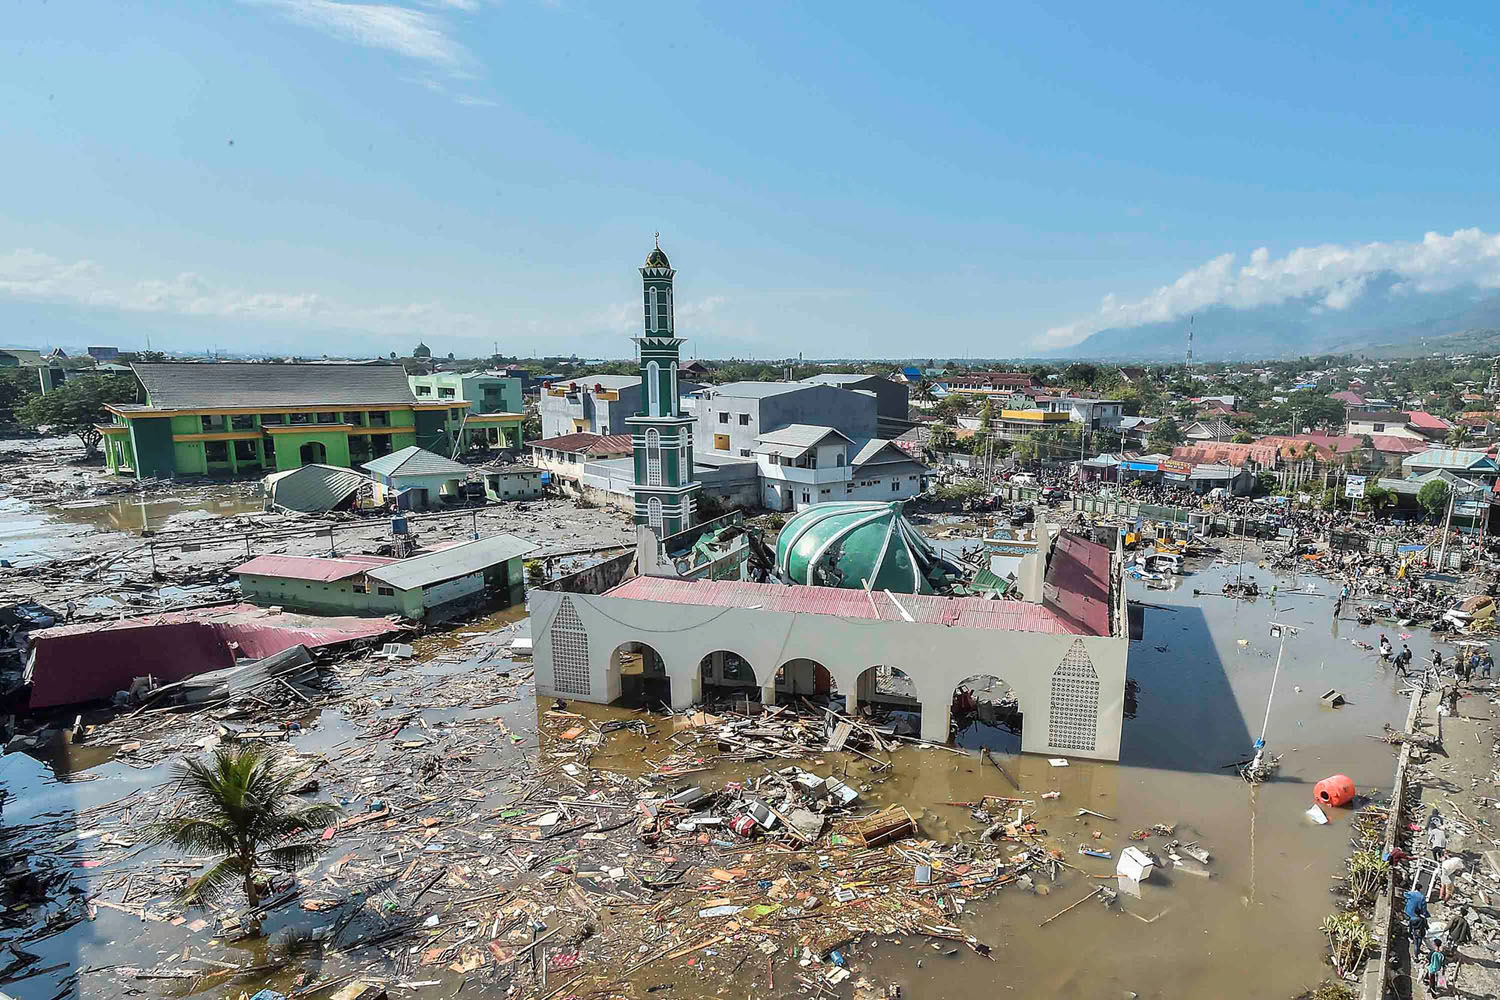
\includegraphics[width=0.7\textwidth]{./Pics/Web/SualwesiTsunami.jpg}
		\caption{Sulawesi Tsunami (Indonesia, 2018).}
	\end{figure}
\end{frame}
\againframe<3>{MotivationFrame}
\begin{frame}{Storm Surge of Hurricane Florence and Michael}
	\begin{figure}
		\centering
	\begin{subfigure}{0.5\textwidth}
		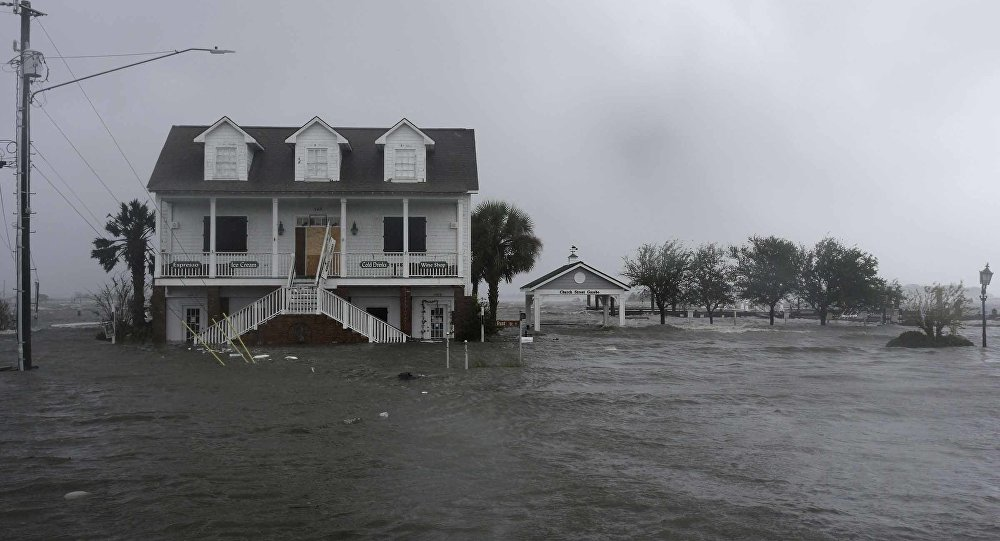
\includegraphics[width=0.9\textwidth]{./Pics/Web/HurricaneFlorence.jpg}
		\subcaption{Florence (U.S.A, 2018)}
		\vspace{0.5cm}
	\end{subfigure}%
	\begin{subfigure}{0.5\textwidth}
		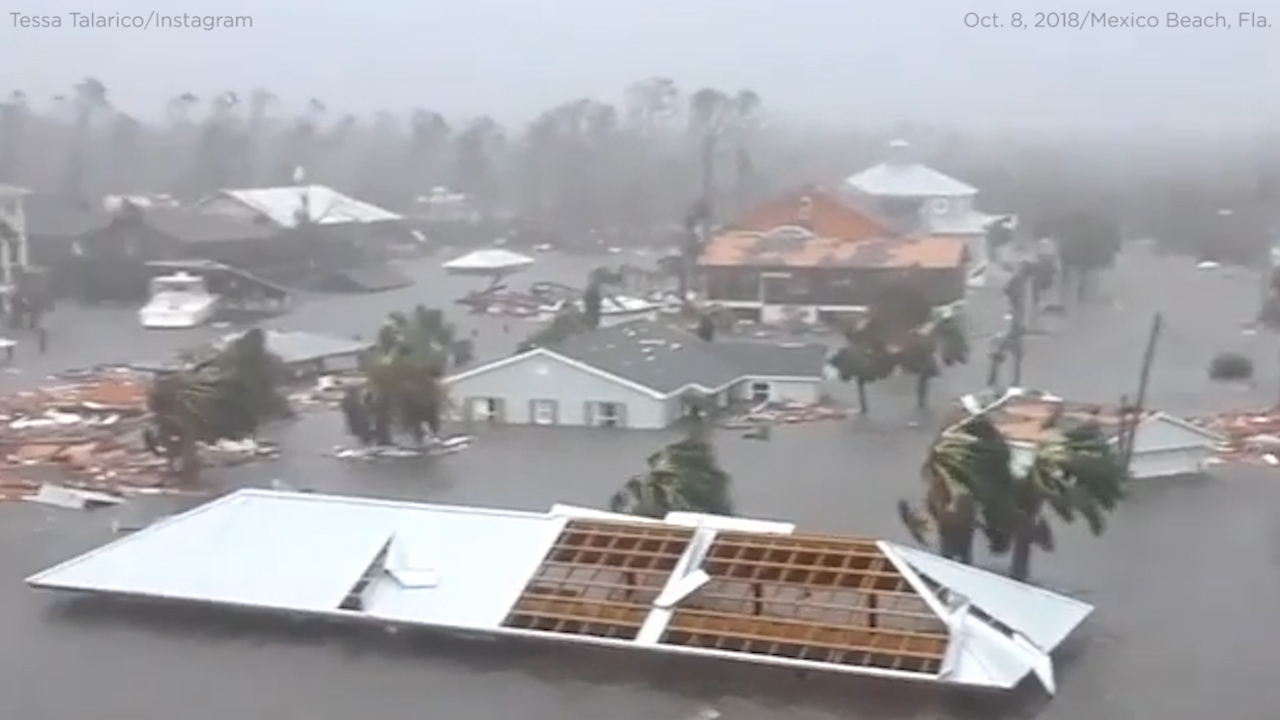
\includegraphics[width=0.9\textwidth]{./Pics/Web/HurricanMichael.jpg}
		\subcaption{Michael (U.S.A, 2018)}
		\vspace{0.5cm}
	\end{subfigure}
\end{figure}
\end{frame}
\subsection{Water Model}
\begin{frame}{Two Dimensional Scenario}
		\begin{figure}
			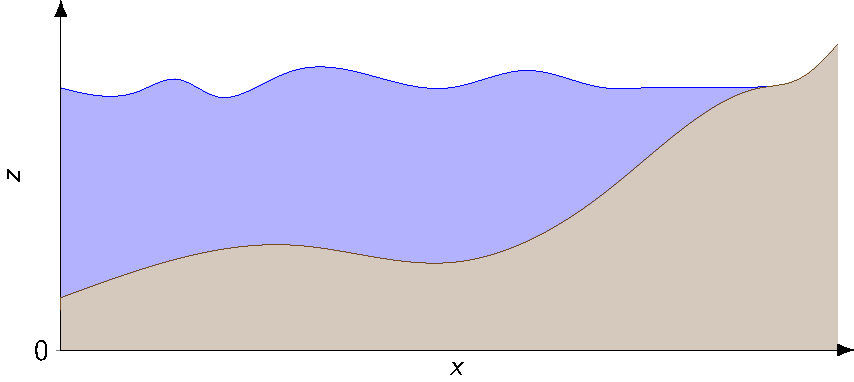
\includegraphics[width=\textwidth]{./Pics/Tex/WaterModel/FressSurface.pdf}
		\end{figure}
\end{frame}

\begin{frame}{Navier-Stokes }
	%Particles, but actualy contain many thousands/millions of particles so that it behaves continuosly
	\begin{figure}
		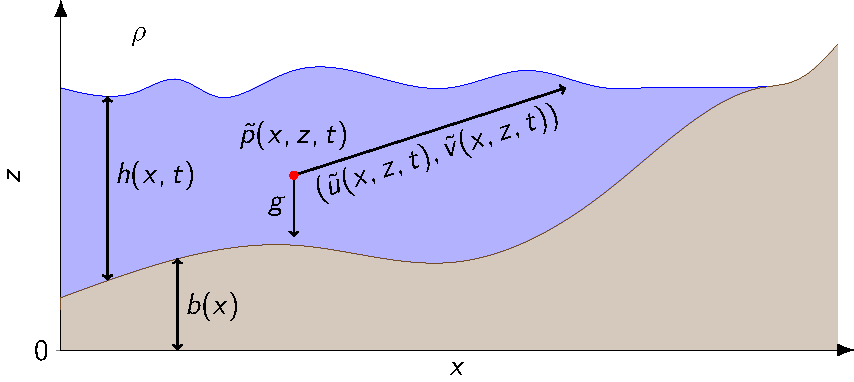
\includegraphics[width=\textwidth]{./Pics/Tex/WaterModel/NavierStokes.pdf}
	\end{figure}
\end{frame}
\begin{frame}{Shallow Water Regime}
	\begin{itemize}
		\pause
		\item Neglect viscosity
		\pause
		\item Shallow water - wavelengths far larger than water depth 
		\pause
		\begin{itemize}
			\item Tsunami wavelengths up to 100s of kilometres
			\item Maximum ocean depth is 11 kilometres
		\end{itemize}
	\end{itemize}
\end{frame}

\begin{frame}{Model Simplification: Serre Equations }
	\begin{figure}
		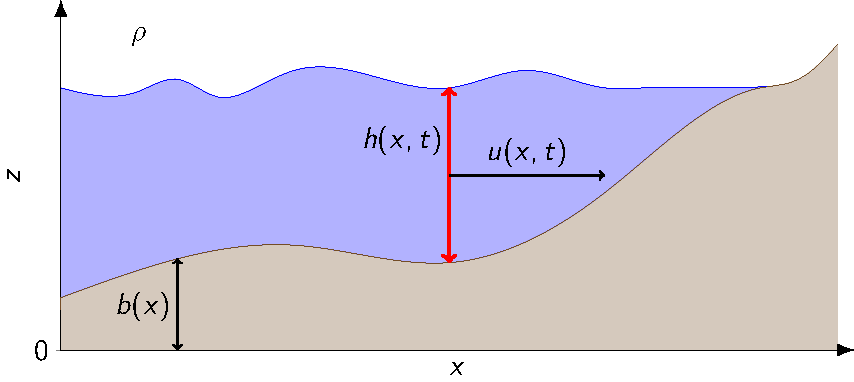
\includegraphics[width=\textwidth]{./Pics/Tex/WaterModel/Serre.pdf}
	\end{figure}
\end{frame}

\begin{frame}{Assumptions}
	\bigbreak
	\pause
	\begin{tabular}{l | c }
		Quantity& Serre Equations\\
		\hline \\
		Particle: $\tilde{u}(x,z,t)$ & $u(x,t)$ \\ &  \\ 
		\pause
		Particle: $\tilde{v}(x,z,t)$ & $u\frac{\partial b}{\partial x} - (z - b)\frac{\partial b}{\partial x}$ \\ &  \\ 
		\pause
		Particle: $\tilde{p}(x,z,t)$& $g \rho \left[h + b - z\right] + \rho \left[h + b - z\right] { \color{green!50!black}\Psi } $ \\& \\ & $+ \frac{1}{2} \rho \left(h^2 - \left[z - b \right]^2\right) { \color{blue} \Phi }$  \\ \hline
	\end{tabular}
	\bigbreak
	where
	\begin{align*}
	&{ \color{green!50!black}\Psi }  = \dfrac{\partial b}{\partial x}\left(\dfrac{\partial u}{\partial t} + u\dfrac{\partial u}{\partial x} \right)  + u^2\dfrac{\partial^2 b}{\partial x^2}, &
	{ \color{blue} \Phi }  = \dfrac{\partial u }{\partial x} \dfrac{\partial u}{\partial x} -u \dfrac{\partial^2 u}{\partial x^2}  - \dfrac{\partial^2 u}{\partial x \partial t} .
	\end{align*}
\end{frame}

\begin{frame}{Equations}
	\begin{subequations}
		\begin{align*}
		&\text{Mass:} && \frac{\partial h}{\partial t} + \dfrac{\partial (uh)}{\partial x} = 0,  \\ \\
		&\text{Momentum:} &&\dfrac{\partial (uh)}{\partial t} + \dfrac{\partial}{\partial x} \left ( u^2h + \dfrac{gh^2}{2} + \dfrac{h^2}{2}{ \color{green!50!black}\Psi } + \dfrac{h^3}{3}{ { \color{blue} \Phi } }  \right )   \\ \\& &&\quad \quad \; \; +  \dfrac{\partial b}{\partial x} \left (gh +   h { \color{green!50!black}\Psi } + \dfrac{h^2}{2}{ { \color{blue} \Phi } }  \right ) = 0.
		\end{align*}
	\end{subequations}
	\begin{align*}
	&{ \color{green!50!black}\Psi }  = \dfrac{\partial b}{\partial x}\left(\dfrac{\partial u}{\partial t} + u\dfrac{\partial u}{\partial x} \right)  + u^2\dfrac{\partial^2 b}{\partial x^2}, &
	{ \color{blue} \Phi }  = \dfrac{\partial u }{\partial x} \dfrac{\partial u}{\partial x} -u \dfrac{\partial^2 u}{\partial x^2}  - \dfrac{\partial^2 u}{\partial x \partial t} .
	\end{align*}
\end{frame}


\section{Method}
\subsection{Introduction}
\begin{frame}{Method}
	\begin{itemize}
		\item When $\Phi = \Psi =0$ we have the Shallow Water Wave Equations
		\pause
		\item Demonstrated utility of Finite Volume Methods for these equations (ANUGA) \\
		\pause
		\item[Goal:] Adapt Finite Volume Methods for the Serre Equations
	\end{itemize}
\end{frame}

\subsection{Finite Volume Method}
\begin{frame}[label=FVM]{Finite Volume Method}
	\begin{itemize}
		\item Conservation law form
		\pause
		\item Finite volume update 
	\end{itemize}
\end{frame}

\againframe<1>{FVM}

\begin{frame}[label=ConLawForm]{Conservation Law Form}
	\begin{equation*}
	{\frac{\partial q}{\partial t}} +  {\frac{\partial}{\partial x}} \left[ f\left(q,{\frac{\partial q}{\partial x}}, {\frac{\partial^2 q}{\partial x^2}}, \dots,{\frac{\partial^n q}{\partial x^n}}\right)\right] + s\left(q,{\frac{\partial q}{\partial x}}, {\frac{\partial^2 q}{\partial x^2}}, \dots,{\frac{\partial^m q}{\partial x^m}}\right) = 0
	\end{equation*}
\end{frame}

\begin{frame}{Equations}
	\begin{subequations}
		\begin{align*}
		&\text{Mass:} && \frac{\partial h}{\partial t} + \dfrac{\partial (uh)}{\partial x} = 0,  \\ \\
		&\text{Momentum:} &&\dfrac{\partial (uh)}{\partial t} + \dfrac{\partial}{\partial x} \left ( u^2h + \dfrac{gh^2}{2} + \dfrac{h^2}{2}{ \color{green!50!black}\Psi } + \dfrac{h^3}{3}{ { \color{blue} \Phi } }  \right )   \\ \\& &&\quad \quad \; \; +  \dfrac{\partial b}{\partial x} \left (gh +   h { \color{green!50!black}\Psi } + \dfrac{h^2}{2}{ { \color{blue} \Phi } }  \right ) = 0.
		\end{align*}
	\end{subequations}
	\begin{align*}
	&{ \color{green!50!black}\Psi }  = \dfrac{\partial b}{\partial x}\left(\dfrac{\partial u}{\partial t} + u\dfrac{\partial u}{\partial x} \right)  + u^2\dfrac{\partial^2 b}{\partial x^2}, &
	{ \color{blue} \Phi }  = \dfrac{\partial u }{\partial x} \dfrac{\partial u}{\partial x} -u \dfrac{\partial^2 u}{\partial x^2}  - \dfrac{\partial^2 u}{\partial x \partial t} .
	\end{align*}
\end{frame}

\begin{frame}{Equations}
	\begin{subequations}
		\begin{align*}
		&\text{Mass:} && \frac{\partial h}{\partial t} + \dfrac{\partial (uh)}{\partial x} = 0,  \\ \\
		&\text{Momentum:} &&\dfrac{\partial (uh)}{\partial t} + \dfrac{\partial}{\partial x} \left ( u^2h + \dfrac{gh^2}{2} + \dfrac{h^2}{2}{ \color{green!50!black}\Psi } + \dfrac{h^3}{3}{ { \color{blue} \Phi } }  \right )   \\ \\& &&\quad \quad \; \; +  \dfrac{\partial b}{\partial x} \left (gh +   h { \color{green!50!black}\Psi } + \dfrac{h^2}{2}{ { \color{blue} \Phi } }  \right ) = 0.
		\end{align*}
	\end{subequations}
	\begin{align*}
	&{ \color{green!50!black}\Psi }  = \dfrac{\partial b}{\partial x}\left( {\color{red}\dfrac{\partial u}{\partial t}} + u\dfrac{\partial u}{\partial x} \right)  + u^2\dfrac{\partial^2 b}{\partial x^2}, &
	{ \color{blue} \Phi }  = \dfrac{\partial u }{\partial x} \dfrac{\partial u}{\partial x} -u \dfrac{\partial^2 u}{\partial x^2}  - {\color{red}\dfrac{\partial^2 u}{\partial x \partial t}} .
	\end{align*}
\end{frame}

\begin{frame}<1>{Conservation Law Form}
	\begin{align*}
	& \frac{\partial h}{\partial t} + \dfrac{\partial (uh)}{\partial x} = 0,  \\ \nonumber \\
	\begin{split}
	\frac{\partial G}{\partial t}  + \frac{\partial}{\partial x} \left( {u} G + \frac{gh^2}{2} - \frac{2}{3}h^3 \left[\frac{\partial {u}}{\partial x}\right]^2 + h^2 {u}\frac{\partial {u}}{\partial x}\frac{\partial b}{\partial x} \right) \\ + \frac{1}{2}h^2 {u} \frac{\partial {u}}{\partial x} \frac{\partial^2 b}{\partial x^2}  - h {u}^2\frac{\partial b}{\partial x}\frac{\partial^2 b}{\partial x^2} + gh\frac{\partial b}{\partial x} = 0 .
	\end{split}
	\end{align*}
	\pause
	with
	\[ G =  h {u} \left(1 + \frac{\partial h}{\partial x}\frac{\partial b}{\partial x} + \frac{1}{2}h\frac{\partial^2 b}{\partial x^2} + \left[\frac{\partial b}{\partial x}\right]^2 \right) - \frac{\partial}{\partial x}\left(\frac{1}{3}h^3  \frac{\partial {u}}{\partial x}\right).\]
\end{frame}
\begin{frame}<2>{Conservation Law Form}
	\begin{align*}
	& \frac{\partial h}{\partial t} + \dfrac{\partial (uh)}{\partial x} = 0,  \\ \nonumber \\
	\begin{split}
	\frac{\partial { \color{red}G}}{\partial t}  + \frac{\partial}{\partial x} \left( {u} { \color{red}G} + \frac{gh^2}{2} - \frac{2}{3}h^3 \left[\frac{\partial {u}}{\partial x}\right]^2 + h^2 {u}\frac{\partial {u}}{\partial x}\frac{\partial b}{\partial x} \right) \\ + \frac{1}{2}h^2 {u} \frac{\partial {u}}{\partial x} \frac{\partial^2 b}{\partial x^2}  - h {u}^2\frac{\partial b}{\partial x}\frac{\partial^2 b}{\partial x^2} + gh\frac{\partial b}{\partial x} = 0 .
	\end{split}
	\end{align*}
	\pause
	with
	\[ { \color{red}G} =  h {u} \left(1 + \frac{\partial h}{\partial x}\frac{\partial b}{\partial x} + \frac{1}{2}h\frac{\partial^2 b}{\partial x^2} + \left[\frac{\partial b}{\partial x}\right]^2 \right) - \frac{\partial}{\partial x}\left(\frac{1}{3}h^3  \frac{\partial {u}}{\partial x}\right).\]
\end{frame}

\againframe<2>{FVM}
\againframe{ConLawForm}
\begin{frame}{Finite Volume Method}
	\begin{figure}
		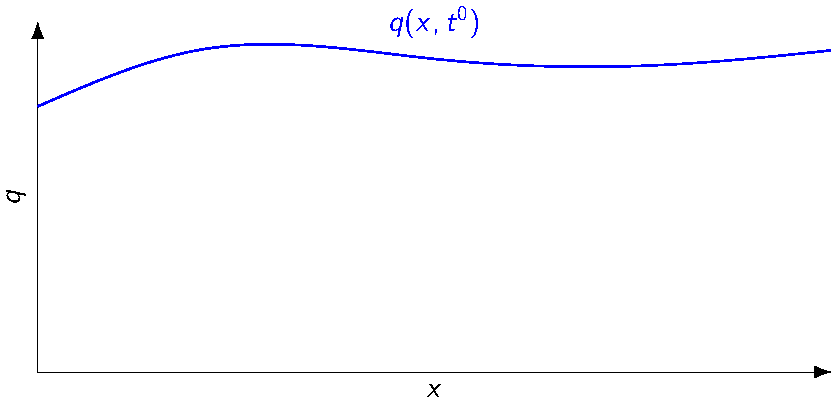
\includegraphics[width=\textwidth]{./Pics/Tex/FVM/Function.pdf}
	\end{figure}
\end{frame}

\begin{frame}{Discretisation}
	\begin{figure}
		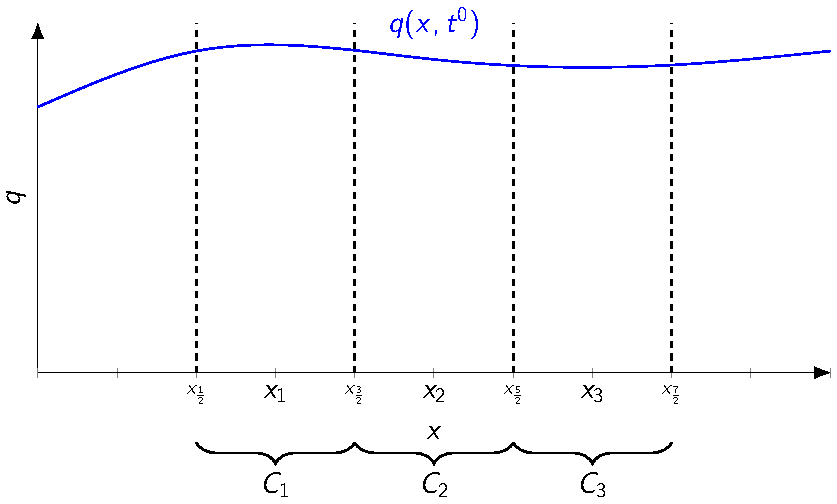
\includegraphics[width=\textwidth]{./Pics/Tex/FVM/Cells.pdf}
	\end{figure}
\end{frame}

\begin{frame}{Update}
	\begin{figure}
		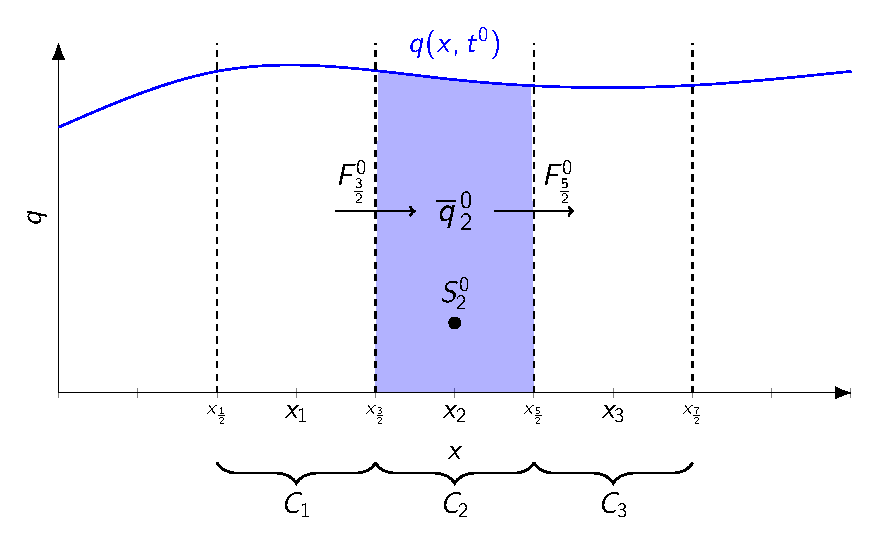
\includegraphics[width=\textwidth]{./Pics/Tex/FVM/TotalFluxInOutSource.pdf}
	\end{figure}
\end{frame}

\begin{frame}{Finite Volume Method}
	\begin{figure}
		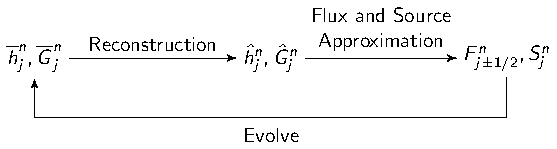
\includegraphics[width=\textwidth]{./Pics/Tex/FlowCharts/FVM.pdf}
	\end{figure}
	%Since $b(x)$ is constant in time its omitted
\end{frame}

\begin{frame}{Require velocity to calculate flux and source}
	However to calculate the flux and source terms we require $u$
	\pause	
	\begin{align*}
	& \frac{\partial h}{\partial t} + {\color{red}\dfrac{\partial (uh)}{\partial x}} = 0,  \\ \nonumber \\
	\begin{split}
	\frac{\partial G}{\partial t}  + \frac{\partial}{\partial x} \left( {\color{red}uG} + \frac{gh^2}{2} - {\color{red}\frac{2}{3}h^3 \left[\frac{\partial {u}}{\partial x}\right]^2} + {\color{red}h^2 {u}\frac{\partial {u}}{\partial x}\frac{\partial b}{\partial x} }\right) \\ + {\color{red}\frac{1}{2}h^2 {u} \frac{\partial {u}}{\partial x} \frac{\partial^2 b}{\partial x^2} } -  {\color{red} h {u}^2\frac{\partial b}{\partial x}\frac{\partial^2 b}{\partial x^2}} + gh\frac{\partial b}{\partial x} = 0 .
	\end{split}
	\end{align*}
\end{frame}

\begin{frame}{Method}
	\begin{figure}
		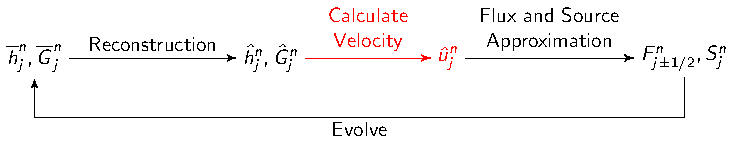
\includegraphics[width=1\textwidth]{./Pics/Tex/FlowCharts/FEVM.pdf}
	\end{figure}
\end{frame}
\subsection{Reconstruction}
\begin{frame}{Reconstruction}
	\begin{itemize}
		\item Determines spatial order of accuracy \\ \pause 
		\item[Goal:] Second-order accuracy %(at least approximate all terms by linear functions) 
	\end{itemize}
\end{frame}
\begin{frame}<1-2>[label=ReconSpaces]{Reconstruction Spaces}
	%Justify discontinuity, continuity
	\begin{tabular}{l | c | c}
		Quantity& Number of &  Reconstructed \\
		 & spatial derivatives &  functions\\
		\hline \pause
		$h$ & zero & linear over cell, discontinuous at edges \\
		$G$ & zero & linear over cell, discontinuous at edges  \\ & & \\
		\pause 
		$u$ & one & quadratic over cell, continuous at edges\\ & & \\
		\pause
		$b$ & two & cubic over cell, continuous at edges \\ 
	\end{tabular}
\end{frame}
\begin{frame}{$\hat{h},\hat{G}$}
	\begin{figure}
		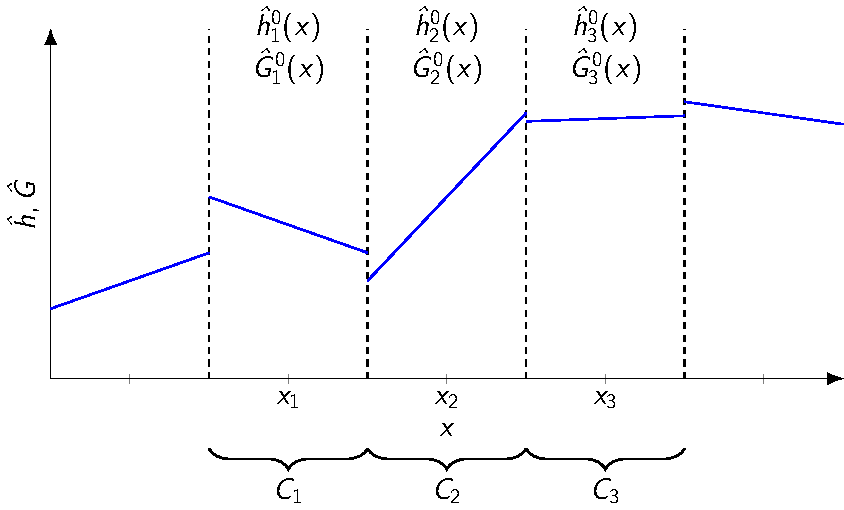
\includegraphics[width=\textwidth]{./Pics/Tex/Reconstructions/P1.pdf}
	\end{figure}
\end{frame}
\againframe<3>{ReconSpaces}
\begin{frame}{$\hat{u}$}
	\begin{figure}
		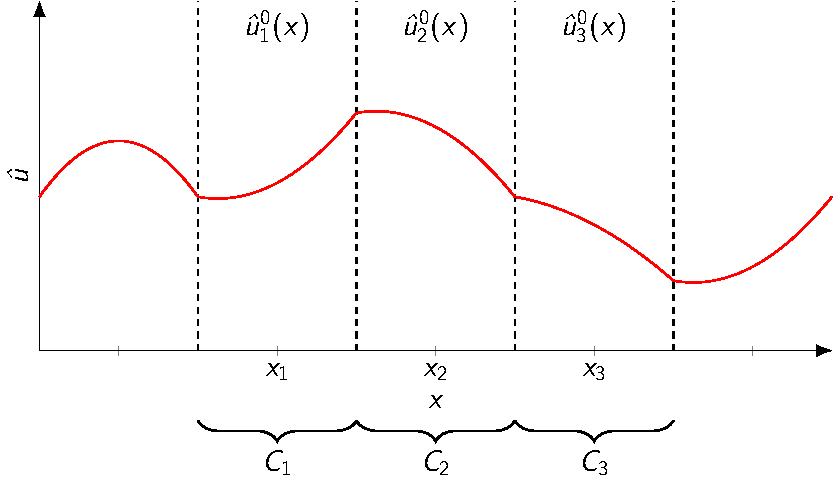
\includegraphics[width=1\textwidth]{./Pics/Tex/Reconstructions/P2.pdf}
	\end{figure}
\end{frame}
\againframe<4>{ReconSpaces}
\begin{frame}{$\hat{b}$}
	\begin{figure}
		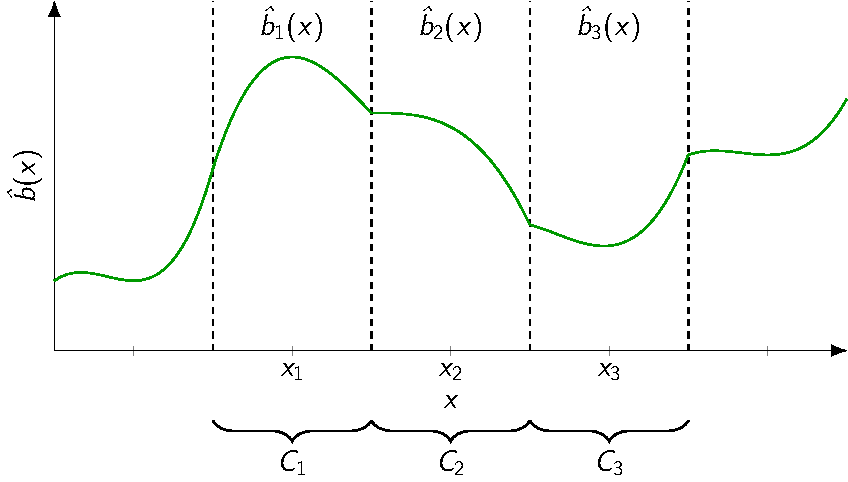
\includegraphics[width=1\textwidth]{./Pics/Tex/Reconstructions/P3.pdf}
	\end{figure}
\end{frame}
\subsection{Calculation of Velocity}
\begin{frame}{Finite Element Calculation of Velocity}
	Finite Element Method to solve:
		\[ G =  h {u} \left(1 + \frac{\partial h}{\partial x}\frac{\partial b}{\partial x} + \frac{1}{2}h\frac{\partial^2 b}{\partial x^2} + \left[\frac{\partial b}{\partial x}\right]^2 \right) - \frac{\partial}{\partial x}\left(\frac{1}{3}h^3  \frac{\partial {u}}{\partial x}\right).\]
	for $u$ given $h$, $G$ and $b$ \\ \bigskip \pause 
	Solves the weak form replacing all quantities with their reconstructions $\hat{h}$, $\hat{G}$ and $\hat{b}$ to get $\hat{u}$
\end{frame}
\begin{frame}{Method}
		\begin{figure}
			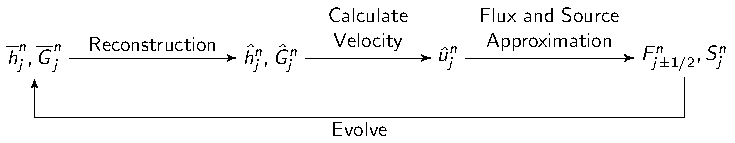
\includegraphics[width=1\textwidth]{./Pics/Tex/FlowCharts/FEVMblack.pdf}
		\end{figure}
\end{frame}

\section{Results}
\begin{frame}[label=valid]{Validation}
	\begin{itemize}
		\item Analytic Solution
		\pause
		\item Experimental Results
	\end{itemize}
\end{frame}
\againframe<1>{valid}
\subsection{Analytic Solution}
\begin{frame}{Soliton Example}
		\begin{figure}
			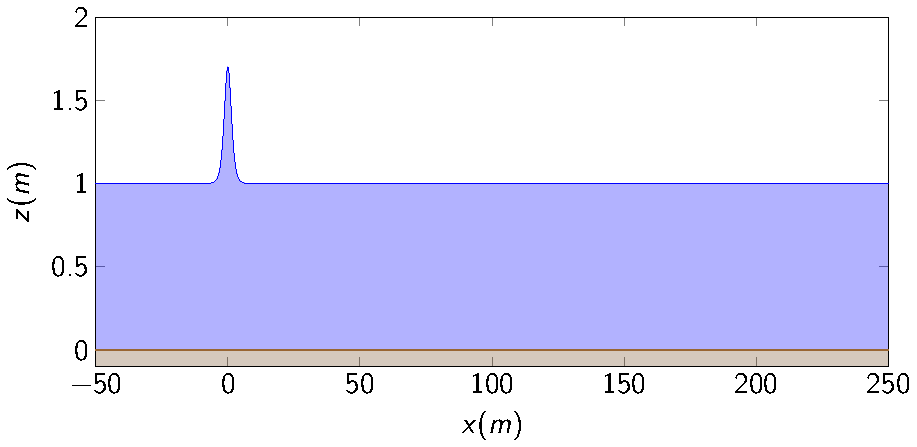
\includegraphics[width=\textwidth]{./Pics/Init/SolitonAnalytict=0s.pdf}
		\end{figure}
		%a_0 = 1, a_1 = 0.7
	
\end{frame}

 \begin{frame}[plain]
 	\begin{tikzpicture}[remember picture,overlay]
 	\node[anchor=north east, inner sep=0pt] at (current page.north east) {%
 		%\movie[height = 0.97\paperheight, width = \paperwidth, loop,showcontrols] {}{./Video/SolitonAnalytic.avi}%
 		% 		\includemovie[
 		% 		poster,
 		% 		text={}
 		% 		]{\paperwidth}{\paperheight}{./Video/SolitonAnalytic.mp4}
 		\includemedia[
 		width=\paperwidth,
 		height=\paperheight,
 		activate=pageopen,
 		addresource=./Video/SolitonAnalytic.mp4,
 		flashvars={source=./Video/SolitonAnalytic.mp4}
 		]{}{VPlayer.swf}
 	};
 	\end{tikzpicture}
 \end{frame}
\begin{frame}{Soliton Equations}
	
		\begin{align*}
		&h(x,t) = a_0 + a_1\text{sech}\left(\kappa \left(x - ct\right)\right), \\  \nonumber \\
		&u(x,t) = c\left(1 - \dfrac{a_0}{h(x,t)}\right), \\
		&b(x) = 0
		\end{align*}
		\pause 
\begin{align*}
&\kappa = \dfrac{\sqrt{3a_1}}{2 a_0\sqrt{\left(a_0 + a_1\right)}}, \\ \\
&c = \sqrt{g(a_0 + a_1)}.
\end{align*}
\end{frame}


\begin{frame}{Numerical Solution $a_0 = 1m$, $a_1 = 0.7m$ }
				\begin{figure}
					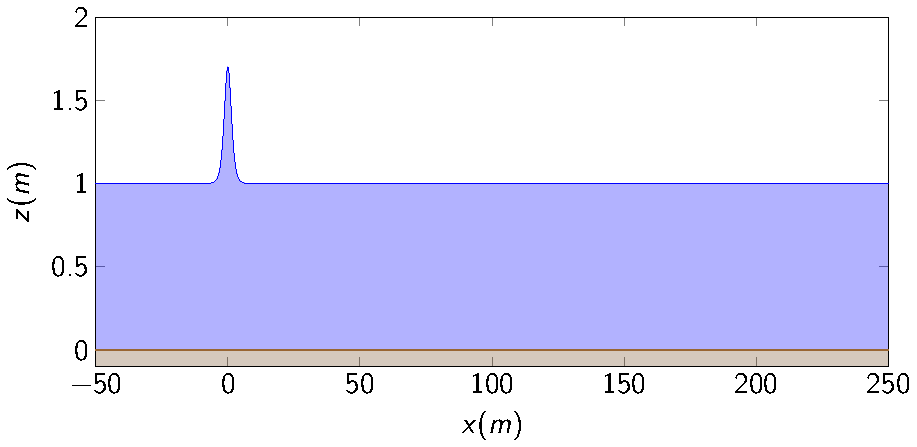
\includegraphics[width=\textwidth]{./Pics/Init/SolitonAnalytict=0s.pdf}
				\end{figure}
\end{frame}
 \begin{frame}[plain]
 	\begin{tikzpicture}[remember picture,overlay]
 	\node[anchor=north east, inner sep=0pt] at (current page.north east) {%
 		%\movie[height = 0.97\paperheight, width = \paperwidth, loop,showcontrols] {}{./Video/SolitonNumerical.avi}
 		% 		 			\includemovie[
 		% 		 			poster,
 		% 		 			text={}
 		% 		 			]{\paperwidth}{\paperheight}{./Video/SolitonNumerical.mp4}
 		\includemedia[
 		width=\paperwidth,
 		height=\paperheight,
 		activate=pageopen,
 		addresource=./Video/SolitonNumerical.mp4,
 		flashvars={source=./Video/SolitonNumerical.mp4}
 		]{}{VPlayer.swf}
 	};
 	\end{tikzpicture}
 \end{frame}

\begin{frame}{Convergence}
		\begin{figure}
			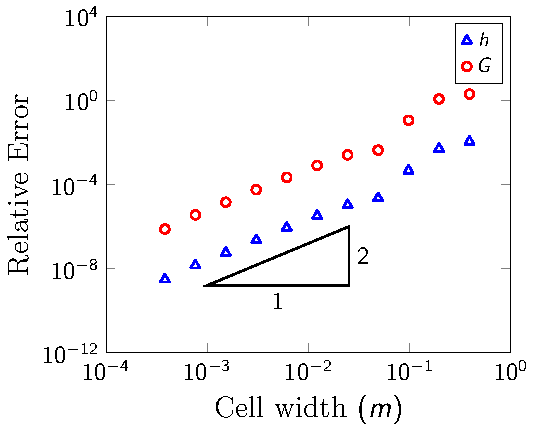
\includegraphics[width=0.75\textwidth]{./Pics/Tex/Soliton/L1/L1.pdf}
		\end{figure}
\end{frame}
\begin{frame}{Conservation}
			\begin{figure}
				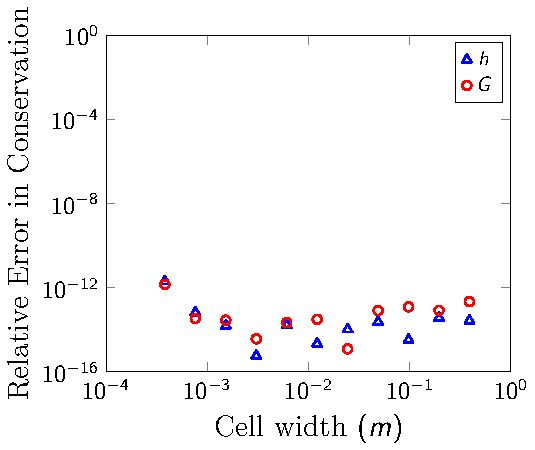
\includegraphics[width=0.75\textwidth]{./Pics/Tex/Soliton/C1/C1.pdf}
			\end{figure}
\end{frame}
\againframe<2>{valid}
\subsection{Experimental Comparison}
\begin{frame}{Synolakis Experiment}
			\begin{figure}
				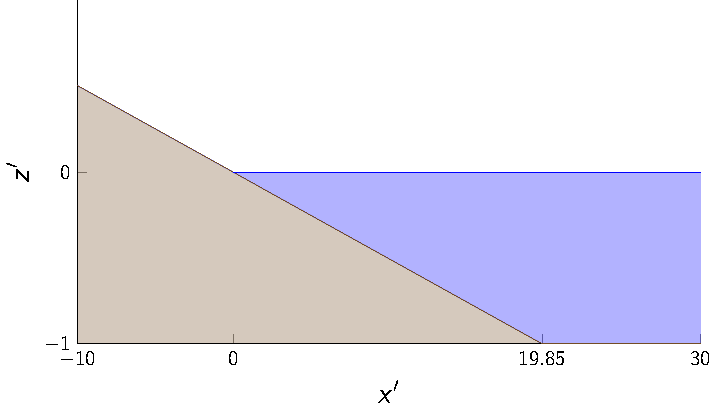
\includegraphics[width=\textwidth]{./Pics/Synolakis/WavetankArtificalPres.pdf}
			\end{figure}
\end{frame}
\begin{frame}{Numerical Solution}
					\begin{figure}
						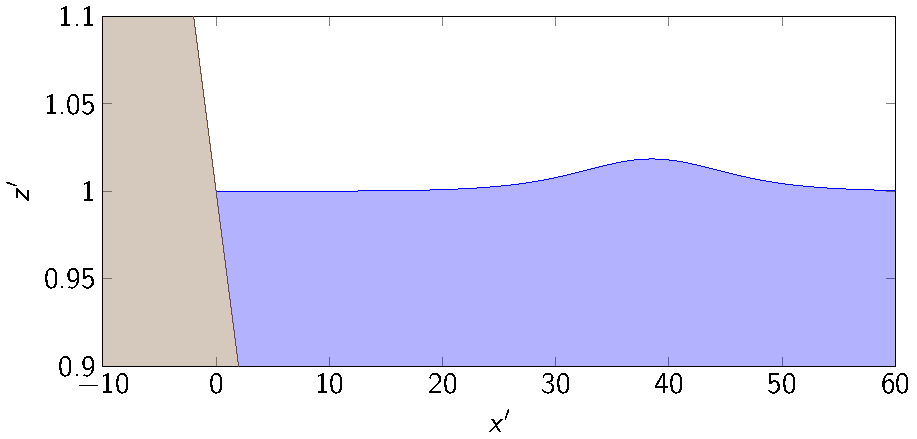
\includegraphics[width=\textwidth]{./Pics/Init/Synolakist=0s.pdf}
					\end{figure}
\end{frame}

 \begin{frame}[plain]
 	\begin{tikzpicture}[remember picture,overlay]
 	\node[anchor=north east, inner sep=0pt] at (current page.north east) {%
 		%\movie[height = 0.99\paperheight, width = \paperwidth, loop,showcontrols] {}{./Video/SynolakisNumerical.avi}%
 		% 			%\includemovie[
 		% 			poster,
 		% 			text={}
 		% 			]{\paperwidth}{\paperheight}{./Video/SynolakisNumerical.mp4}
 		\includemedia[
 		width=\paperwidth,
 		height=\paperheight,
 		activate=pageopen,
 		addresource=./Video/SynolakisNumerical.mp4,
 		flashvars={source=./Video/SynolakisNumerical.mp4}
 		]{}{VPlayer.swf}
 	};
 	\end{tikzpicture}
 \end{frame}

\begin{frame}{Comparison $t'=30$}
		\begin{figure}
			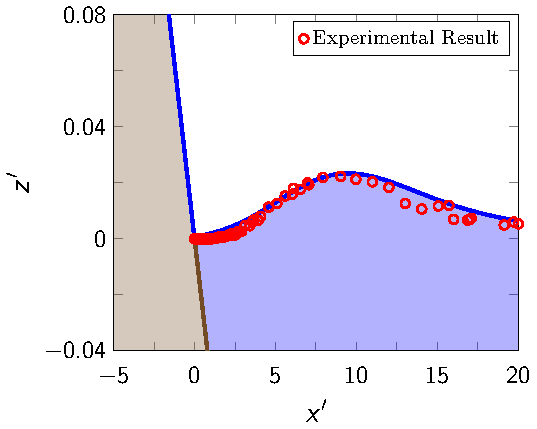
\includegraphics[width=0.75\textwidth]{./Pics/Synolakis/t=30s.pdf}
		\end{figure}
\end{frame}

\begin{frame}{Comparison $t'=40$}
	\begin{figure}
		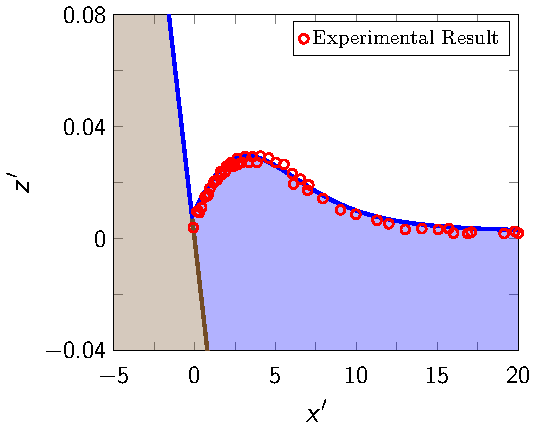
\includegraphics[width=0.75\textwidth]{./Pics/Synolakis/t=40s.pdf}
	\end{figure}
\end{frame}

\begin{frame}{Comparison $t'=50$}
	\begin{figure}
		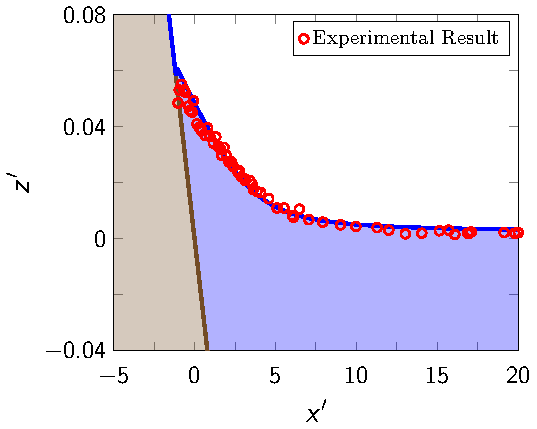
\includegraphics[width=0.75\textwidth]{./Pics/Synolakis/t=50s.pdf}
	\end{figure}
\end{frame}

\begin{frame}{Comparison $t'=60$}
	\begin{figure}
		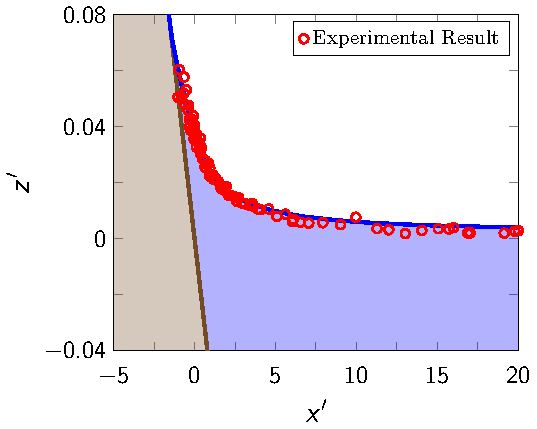
\includegraphics[width=0.75\textwidth]{./Pics/Synolakis/t=60s.pdf}
	\end{figure}
\end{frame}

\begin{frame}{Comparison $t'=70$}
	\begin{figure}
		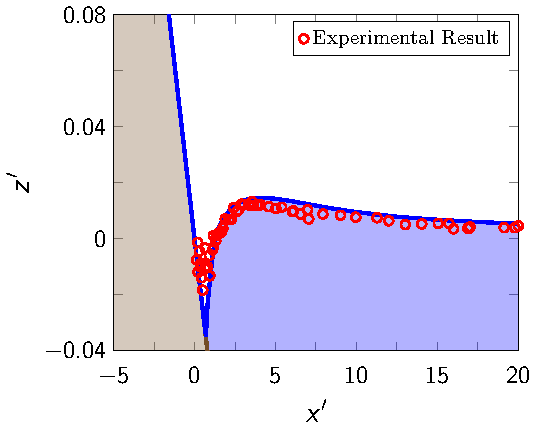
\includegraphics[width=0.75\textwidth]{./Pics/Synolakis/t=70s.pdf}
	\end{figure}
\end{frame}

\begin{frame}{Conclusion}
	Finite Element Volume Method for The Serre Equations
	\begin{itemize}
		\item Second-order accurate
		\pause 
		\item Conservative
		\pause
		\item Reproduces analytic solutions
		\pause
		\item Reproduces experimental results
	\end{itemize}
\end{frame}

\begin{frame}{}
	\centering \Huge Thanks!
\end{frame}

\end{document}